\section{Chapter of Research} 

\section{Introduction}

Assistive technology designed to enable communication for non-verbal disabilities is currently available in the form of software. Special communication apps are used to help speech disabled children communicate via tablets and smart devices. Parents try to limit access to other features on the tablet by locking the device to be used only with the communication app. Through observation while visiting schools and sitting in classrooms, we noted that this causes frustration to the children although it was designed to make their lives easier. we identified a need for a stand-alone device that serves the purpose of communication without offering any other features.

Children with non-verbal autism use a form of sign language called Makaton\footcite{Makaton}. Makaton is a set of action words a child signs to communicate his/her feelings and needs. The focus of the study is to design a hand gesture recognition system to translate Makaton sign language action words to text and speech. 

There are two approaches in research for sign language hand gesture recognition. First approach is using computer vision and the second is using data gloves. Computer-vision hand gesture recognition for the purpose of translating sign language relies on cameras for recognition and therefore, must be paired with smart devices to operate. Data gloves, however, have potential to operate independently from a smart device. Consequently, data gloves recognition is the chosen method to translate sign language hand gestures for this study. 

A Data glove is a wired interface with certain tactile or other sensory units attached to the fingers or joints of the glove, worn by the user. Tactile switches, optical goniometer or resistance sensors measure the bending of different joints which determine if a hand is open or closed and if finger joints are straight or bent. The orientation of the hand can be described in terms of two orthogonal directions—the facing of the palm, and the direction to which the hand is pointing. These results are mapped to unique gestures and are interpreted by a computer. 

Glove based sign language recognition systems have been reported to offer a wider vocabulary and better recognition accuracy than computer vision systems. Nevertheless, the enormity of the sign language library makes it very difficult to find a match within large vocabulary data bases\footcite{Premaratne2010}. Another drawback is the limited manoeuvrability due to wires connecting the gloves to the computer. 

In this study, we use a limited vocabulary of ten action words signs using a wireless and standalone data-glove which has sensors placed to monitor the flexing of fingers to get accurate input information of hand gestures. Recognition modules are based on hand shapes and orientation rather than position or dynamic movement recognition. We have simplified recognition in an attempt to reduce the hardware, making the data glove simpler to run, easier to wear and cheaper to produce. 
In this chapter, we demonstrate how these issues are explored through gained feedback from carers of non-verbal autistic participants about their use of the data glove and how it affected their daily communication. 

This study is part of a program to develop and produce an affordable and accessible data glove that translates sign language to text and speech, facilitating daily communications between individuals with speech disabilities and the general public. 

\section{Background}

Since the 1980s, computer vision and data gloves have been used to recognize hand gestures for the purpose of translating sign language. Hand shapes are one of the primitives of sign language and reflect the information of hand configuration. They are known to be very stable and can be used to distinguish most signs\footcite{Fang2003}. 

Even with advancements in computer vision, glove based sign language recognition offers the widest vocabulary and the best possible recognition accuracy. However, no recent such system has been reported with very high accuracy\footcite{Premaratne2010}, possibly because researchers are more focused on vision based systems. 

There are many versions of the data glove that translate sign language to text or speech. Most of these gloves rely on a smart device for output and perhaps none have moved beyond prototyping. There is almost no published work showing evidence of sign language data gloves being tested by speech-disabled participants for daily communication. This is possibly due to the complex programming and hardware required. In this section, we briefly highlight some examples of the sign language translating Data Gloves.

One of the earlier advanced systems to convert gesture to speech was demonstrated by Fels and Hinton\footcite{Fels1993}. They used a Data Glove in 1992 to convert hand gestures to speech via a speech synthesizer. Their Glove-Talk vocabulary consisted of 66 root words, each with up to six different endings. The total size of the vocabulary was 203 words. Most of these hand shapes represent the ASL alphabet. They also utilized orientation differences in the hand shapes for semantically opposite words such as ``come'' and ``go'' which have a 180 degree orientation difference. Various endings for words were formed through different hand movements. 

Liang and Ouhyoung also used the DataGlove to develop a Taiwanese sign language recognition based on Hidden Markov Models (HMM) and integrated statistical approach used in computational linguistics\footcite{Liang1998}. They utilized specific cues used in Taiwanese Sign Language in order to develop the system. There are 51 fundamental postures in Taiwanese Sign Language. Most gestures mainly contain only one posture, for example, ``I'', ``you'', ``who'', etc., while gestures with multiple postures are also used, such as, ``originally'', ``father'', ``mother'', ``thank'' and ``good-bye''. 

This system was designed to recognize large set of vocabularies in a sign language by recognizing constructive postures and context information. They had a 250 word vocabulary. It could classify 51 static gestures in 6 orientations. They reported that a user dependent system classifying in real- time with an accuracy of 80\%.

In 2011, Oz and Leu developed an American Sign Language (ASL) recognition system based on the Cyberglove\texttrademark sensor glove and artificial neural networks (ANNs) to translate ASL words into English\footcite{Oz2011}. The overall structure of the proposed system consists of a sensory glove and a motion tracker. The data stream from these devices is received and segmented by a velocity net- work with noise reduction and feature extraction followed by a word recognition network. The gesture features extracted from the raw data are then sent to a decoder of the recognition system. The final outcome of the system is to produce voice of the recognized ASL words with a speech synthesizer. 

Their goal was to continuously recognize ASL signs using the glove in real time. They trained the ANN model for 50 ASL words with a different number of samples for every word and the classification results achieved 90\% accuracy which demonstrated that their used successfully for isolated word recognition. They also concluded that some gestures in ASL required that both the right and left hands be manipulated simultaneously by applying the proposed model but with two data gloves and more motion trackers. Although the ANN model was very successful, it never went past the research phase and no plans were made for it to go into production. 

Looking at all previous successful work in this field, we were motivated to introduce this technology to the assistive wearables and healthcare innovation markets and give a chance to speech disabled individuals to try it and use it. 

\section{Method}

Our system has been programmed to identify a limited vocabulary of ten signs based on ten right hand postures and three orientations using an accelerometer data glove to get accurate input information. Failure to detect/identify the gesture will result in no words being spoken. The accelerometer was also used to differentiate between when the glove is being used to sign or to play. When the glove is static it starts processing. In signs using both hands, only the right hand was programmed. This was effective because in signs using both hands, either both hands are the same or one hand stays motionless in holding one position, while the other hand makes the sign. A good example is dance, where the left hand is static while the right hand motions the sign. Another example is play and happy. In both signs, the right and left hand have the same gesture. Two different conversation scenarios were written for the participants where they can communicate using the ten previously programmed actions words. 

Hard coded words were: 

\begin{itemize}
  \item Yes
  \item No
  \item OK
  \item Play
  \item Dance
  \item Colour
  \item Happy
  \item Hungry
  \item Eat
  \item Drink
\end{itemize}

Two participants with non-verbal autism (boys ages 9 and 12) were recruited. Selection criteria was based on the familiarity with sign language according to attending speech therapists recommendations. The training session consisted of 2 hour long task (described below) and broken into four 15 minute segments. Participants were shown videos of the signs, and trained together with the researcher and their speech therapist. Speech therapists'' role was to help the researcher communicate with the participants and provide feedback based on observation. Participants started getting familiar with how the glove worked within half an hour of being introduced to it. Video documentation of the participants using the glove was recorded. Usability feedback from the participants, parents and therapists was noted. 

\section{Task}

A dialogue has been drafted between the therapist and the participant for two simple real life scenarios. The therapists would ask the questions and the participant would sign the reply using the data glove. Words appear on the small screen and are spoken out loud through the speaker on the data glove as in Figures \ref{fig:examplegestures} and \ref{fig:examplegestures2}. The therapist would then move to the next line in the dialogue. This dialogue is an example of a conversation speech disabled individuals engage in every day. 

\subsection{Task I - Participant A - Playtime Dialogue}

\begin{figure}
    \centering
    \begin{subfigure}{.4\linewidth}
        \centering
        \setlength\figureheight{\linewidth}
        \setlength\figurewidth{\linewidth}
        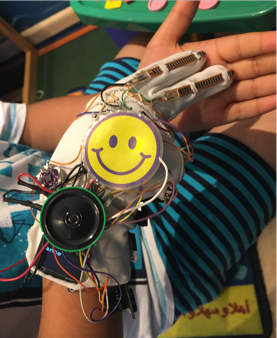
\includegraphics{./assets/img/Dance}
        \caption{Dance}
        \label{fig:dance}
    \end{subfigure}
    \hspace{1cm}
    \begin{subfigure}{.4\linewidth}
        \centering
        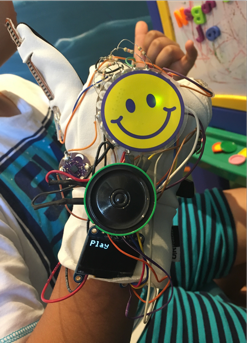
\includegraphics{./assets/img/Play}
        \caption{Play}
        \label{fig:play}
    \end{subfigure}
    \caption{Examples of a test subject making hand gestures while wearing the Data Glove}
    \label{fig:examplegestures}
\end{figure}

\textbf{Data glove pre-programmed Makaton sign language vocabulary:}

\begin{itemize}
  \item Yes
  \item No
  \item OK
  \item Play (Verb)
  \item Dance (Verb)
  \item Colour (Verb)
  \item Happy
  \item Hungry
  \item Eat (Verb)
  \item Drink (Verb)
\end{itemize}

\textbf{Script:}

\begin{description}
  \item Hello! So what are you doing? How was your day so far?
  \item \textit{[...Conversation progresses...]}
  \item Let's do something else? What would you like to do?
  \item \textit{[Subject replies with an activity]}
  \item Really you like to \textit{[insert activity]}?! Do you have any ideas?
  \item \textit{[Subject mimes one of the sign language activities]}
  \item And how does that make you feel?
\end{description}

\subsection{Task II - Participant B - Restaurant Dialogue}

\begin{figure}
    \centering
    \begin{subfigure}{.4\linewidth}
        \centering
        \setlength\figureheight{\linewidth}
        \setlength\figurewidth{\linewidth}
        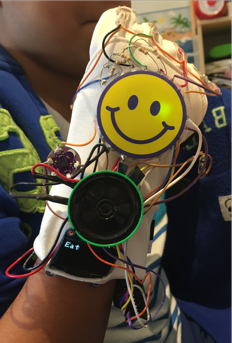
\includegraphics{./assets/img/Eat}
        \caption{Eat}
        \label{fig:eat}
    \end{subfigure}
    \begin{subfigure}{.4\linewidth}
        \centering
        \setlength\figureheight{\linewidth}
        \setlength\figurewidth{\linewidth}
        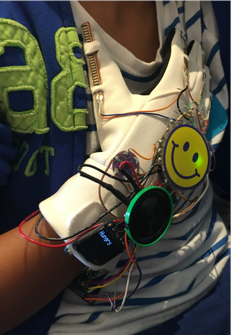
\includegraphics{./assets/img/Hungry}
        \caption{Hungry}
        \label{fig:hungry}
    \end{subfigure}
    \caption{Examples of a test subject making hand gestures while wearing the Data Glove}
    \label{fig:examplegestures2}
\end{figure}

\textbf{Data glove pre-programmed Makaton sign language vocabulary:}

\begin{itemize}
  \item Yes
  \item No
  \item OK
  \item Happy
  \item Hungry
  \item Eat (Verb)
  \item Drink (Verb)
\end{itemize}

\textbf{Script:}

\begin{description}
  \item Hey, do you want to go to a restaurant?
  \item \textit{Yes}
  \item Cool, let's get going!
  \item What will you order?
  \item \textit{[Subject replies with food item]}
  \item Do you want to use the bathroom before we go?
  \item \textit{[Yes/No]}
\end{description}

\section{Feedback} 

Performance feedback was very good, where 4 out of 5 attempts resulted in accurate output. Majority of feedback mainly related to power issues where the glove sometimes got stuck or didn't respond when the battery was running low. Occasionally, the glove had major delays. Battery lasted about two and a half hours. 

Feedback from participants was conveyed through observation and communicated by their therapist. This method is generally used in studies, where users are unable to communicate, or are unable to process information due to their impairment\footcite{Lazar2010} in which case, caregivers and family members were used as the primary information source. 

The participants' feedback was mostly related to glove design and hardware enclosure. Participants expressed that the glove was bulky and felt a little intimidated by the exposed wires. They felt that the glove was uncomfortable to wear and had difficulties bending their fingers. Sometimes glove delays caused frustration amongst the participants because they thought it was their fault. Video documentation took so long that it started to look like it was rehearsed at the end. 

The researcher's observation was that participants wanted to use the glove for other things while wearing it, like playing or holding things\footnote{As in Figure \ref{fig:examplegestures2}}. This affected the output of the glove and programming had to be revisited during the testing phase. A quick solution to get through the testing session was to set the glove to process gestures only when the accelerometer registered an upright position. Other solutions will be discussed below. 

\subsection{Results}

The testing demonstrates that the system is capable of translating sign language to text and speech with an accuracy rate of 80-85\%\footnote{Testing video URL: https://youtu.be/imf5JiCfGrc} and about 15\% of attempts resulting in no words being spoken due to failure to detect the gesture. Reasons for failed attempts is due to the fact that signs vary in time and speed, even with the same user, where slight changes of speed and position of hands occur\footcite{Premaratne2010}. Also, the similarity between some signs sometimes makes it difficult to distinguish them. The fact that the users were playing and signing at the same time while wearing the glove added to this confusion. 

Another factor that affected the results was that participant B had lower motor abilities and therefore was not able to bend his fingers all the way. This threw the glove off recognition ranges for some gestures.

\subsection{Conclusion}

A revised design is being developed based on the feedback of this study. 

Improvements include design, hardware as well as software reconfiguration. 

\textbf{Design:}

Exposed hardware was very intimidating for the children and discouraged them from using the glove.

Glove design has to be revised to be more user friendly. Hardware enclosure has to be redesigned and embedded in the textiles. Custom glove pattern is underway to house the sensors in channels and enclose the hardware in the inner lining of an improved glove design. This new design insures that the circuit is protected as well as insulated from skin contact. Stretchable fabric will be used to make finger movements more flexible and insure easier bending of fingers for small children and children with weak motor development which is common in autism. For safety, fireproof, non-conductive material will be used to house the circuit and insulate the glove.

\textbf{Hardware:} 

Tugging wires was a major issue in this study. 

The Hardware needs to be further reduced and enhanced. The Arduino Lilypad\texttrademark micro-controller is to be replaced by Raspberry Pi Zero. This will further reduce the cost of the hardware to half as well as enhance the performance and battery life. Raspberry Pi also has a built-in text to speech synthesizer which will allow us to eliminate the Emic2 text-to-speech chip from the circuit making the glove more usable. It would also reduce the cost significantly. The accelerometer will be replaced with a gyroscope. A gyroscope will expand feedback from angles and orientation to cover full gesture motions in the 3D space, giving us more data to process and the ability to recognise dynamic gestures. 

I would also like to:
\begin{itemize}
    \item Add a button to switch between training mode and pre-programmed mode. 
    \item Add a button to tell the glove when to process for children who want to keep wearing it. 
    \item Make all hardware removable from glove to be able to wash it. 
    \item Encapsulate circuit to make it water proof. 
    \item Equip the glove with a BLE (Bluetooth\texttrademark Low Energy) chip to provide connectivity with a smart device for training mode. 
\end{itemize}

\textbf{Software:}

Delays in processing was due to the variance in hand gestures between the pre-programmed signs the signer's abilities. Errors occurred because the glove was being used for other activities and didn't have an indication of when to start or stop processing. 

Make the software personal to enhance accuracy is to propose a training mode. Training mode would enable users to upload their own sign language mapped to their individual motor abilities. For that, the glove needs to be paired with machine learning software to store and output gesture classifiers. Enabling users to upload their own version of sign language makes this data glove accessible to everyone who needs it regardless of which sign language library they use. It will also allow children who do not follow a standard sign language library to customize their hand gestures and be able to communicate with the general public, who are unfamiliar with sign language. 

Pair with IBM WATSON\texttrademark APIs for speech translation to other languages. This would make the glove universal and usable in any country breaking yet another language barrier.

\subsection{Future Work}

Based on engagement in the field and taking part in various assistive technology events, it has become evident that there are many different application to the data glove which was designed for this study.

Data gloves for Sign language communities:

\begin{itemize}
    \item Hearing impaired or hard of hearing can use this data glove for their daily communication. 
    \item Empowering professionals with speech disabilities/hearing impairments to conduct meetings, give talks, or go on business trips without the need to hire a translator/interpreter. 
    \item Enabling children with non-verbal disabilities to interact with their peers in integrated classroom. 
    \item Stroke survivors who have limited motor abilities and are not familiar with sign language can train the glove to customised hand gestures. 
    \item This glove can also be used as an educational tool to teach children sign language. 
    \item Accessibility units at airports can utilise the glove for it''s translation features.
    \item Companies who wish to make to transition to become fully inclusive can provide the glove to enable their employees who have speech disabilities. 
\end{itemize}

\textbf{Data Glove applications in other fields:}

Data Gloves are no longer limited for use in computer human interaction. While some Data Gloves are designed for interacting with a computer for gaming and other natural like communication, other Data Gloves are used primarily for 3D motion capture in the motion picture industry as well as some being used for healthcare applications such as the monitoring of vital signs, to physiotherapy on injured or healing hands and fingers\footcite{Premaratne2010}. 

Today, ASL and many sign languages around the world see continuously being interpreted using either vision (with and without markers) or glove based systems as new technology develops. This trend will continue until it results in a highly reliable system in which, the mute and deaf would feel more natural to express their feelings like their able counterparts\footcite{Pavlovic1997}.





